\chapter{Evaluation}
\section{iperf3}

\section{Test Results}
\begin{figure}[h]
	\centering
	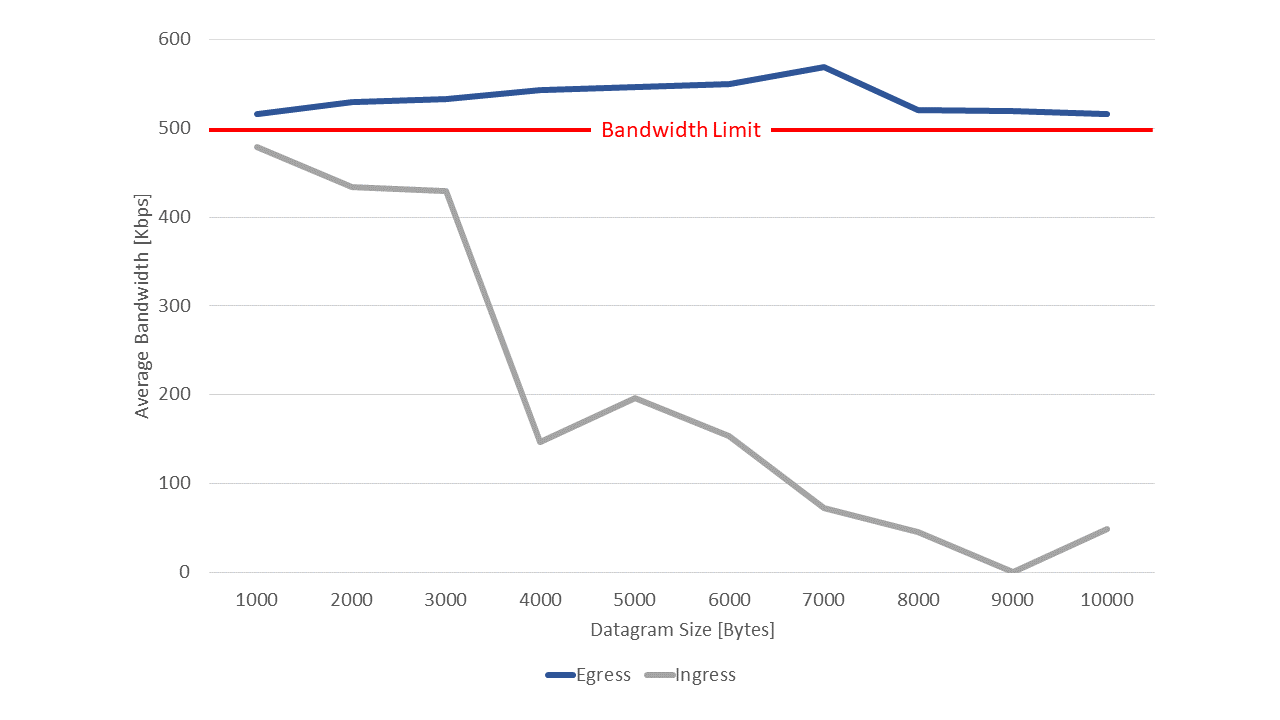
\includegraphics[width=\textwidth]{img/Evaluation-Bandwidth.png}
	\caption{Evaluation of the Bandwidth}
	\label{Evaluation of the Bandwidth}
\end{figure}

\begin{figure}[h]
	\centering
	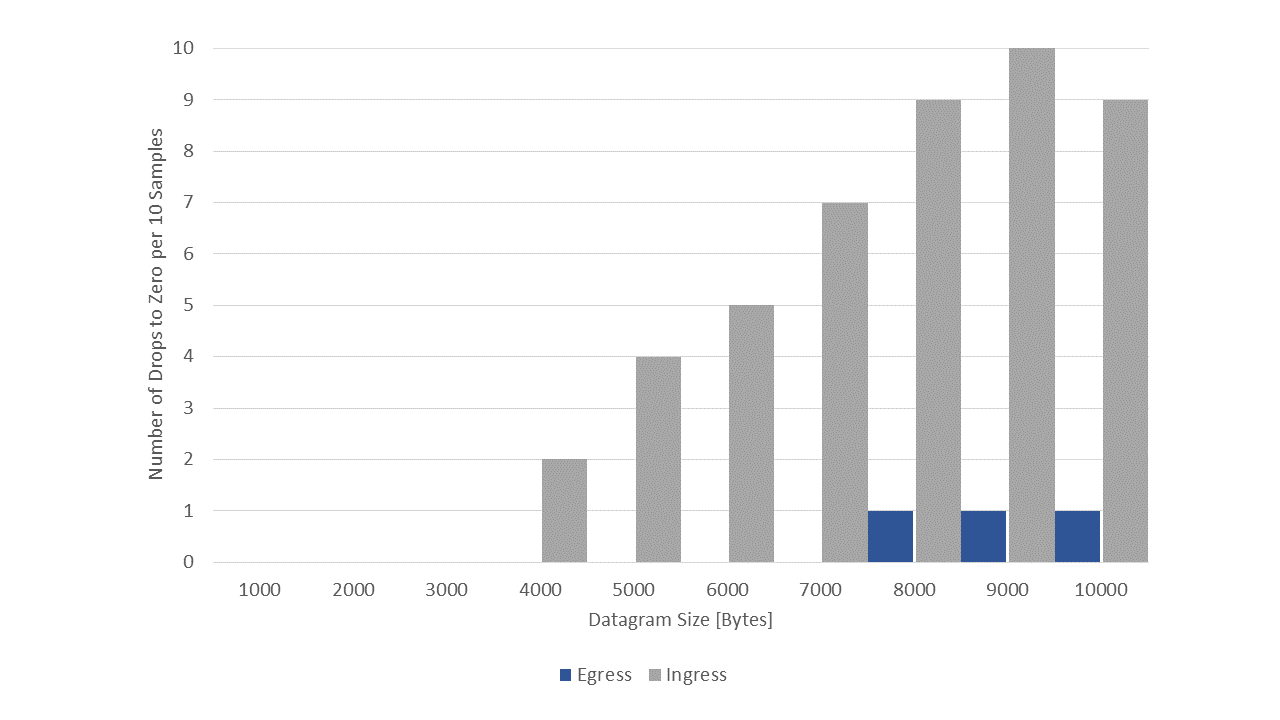
\includegraphics[width=\textwidth]{img/Evaluation-Zeros.png}
	\caption{Evaluation of the Bandwidth Drops}
	\label{Evaluation of the Bandwidth Drops}
\end{figure}

\subsection{Egress Traffic}



\subsection{Ingress Traffic}


%Note: 
%Ingress test: iperf3 -c 192.168.17.129 -u -b 2Mbit -l 1000 -R
%Egress test: iperf3 -c 192.168.17.129 -u -b 2Mbit -l 1000
%important is the -l option that defines the buffer size (KB). otherwise ingress traffic will have one initial burst and then drop to 0

%https://github.com/esnet/iperf/issues/457